% Tutto quello riguardante il progetto andrà in questo capitolo

\chapter{Il progetto}\label{chap:project}
\note{Aiuto i tempi verbaliii! Al futuro? Passato? mi metto in prima persona?}
\section{Presentazione progetto}
Il progetto proposto dall'azienda per il lavoro di stage consiste nel progettare e sviluppare un prototipo di applicazione chat per dispositivi mobili. L'applicativo si dovrà allineare per funzionalità alla soluzione già disponibile in ambiente web e, per quanto riguarda la grafica, al progetto ancora in sviluppo di riprogettazione dell'omonimo modulo Teamwork.
L’applicativo verrà sviluppato con tecnologia React Native, in due varianti per Android e iOS.

\section{Interesse aziendale}
L'applicazione Teamwork sviluppata si appoggerà al software OpenChat, modulo open source \mmh{(disponibile su GitHub all'indirizzo https://github.com/ZeXtras/OpenChat)}{footnote?} sviluppato da Zextras disponibile come Zimlet su Zimbra solo se si dispone del core Zextras.
L'azienda prevede di ottenere dal lavoro di questo stage un prototipo con almeno le funzionalità base di OpenChat su mobile così da:
\begin{itemize}
	\item verificare l'effettiva utilità del progetto;
	\item studiare le migliori soluzioni progettuali per un'ambito \unsure{non ancora toccato} dai prodotti già sviluppati;
	\item validare le tecnologie utilizzate o, aventualmente, proporre altri framework di sviluppo;
	\item ampliare e/o modificare le proprie UX guidelines in base alle differenze tra mobile e desktop.
\end{itemize}


\section{Piano di lavoro}
Lo stage concordato con l'azienda verrà portato avanti da due stagisti e, per ognuno, prevede un lavoro di 320 ore così suddivide:
\begin{itemize}
	\item Formazione (40h): introduzione a Zimbra, Zextras, agli strumenti e procedure aziendali; inoltre un consulente esterno provvederà alla formazione sulle tecnologie da utilizzare per il progetto, quali React Native ed Expo a cui anche l'azienda si interfaccia per la prima volta;
	\item  Progettazione UX (40h): studio e realizzazione di alcuni wireframe dell'app prendendo spunto dall’attuale sistema di chat sviluppato per il web;
	\item Progettazione architetturale (40h): progettazione dell’architettura client/server necessaria per l’implementazione dell'applicazione seguendo le bozze dell’UX;
	\item Implementazione (200h): sviluppo dell’applicazione con l’obiettivo di raggiungere un
	prototipo funzionante.
	
\end{itemize}

\section{Pianificazione di progetto}
Successivamente al periodo di formazione è stato pianificato più in dettaglio il lavoro da svolgere. Le otto settimane di stage sono state suddivise in quattro sprint di due settimane ognuno, riuscendo così a sincronizzare il lavoro con gli sprint dei progetti in corso. \\ Sempre con l'obbiettivo di \unsure{simulare} il metodo lavorativo dell'azienda, è stata associata una versione di release per ognuno dei quattro sprint decisi. \postit{le loro sono vere release le nostre no ovviamente!} \\
I quattro sprint si suddividono così:
\begin{figure}[H] 
	\centering
	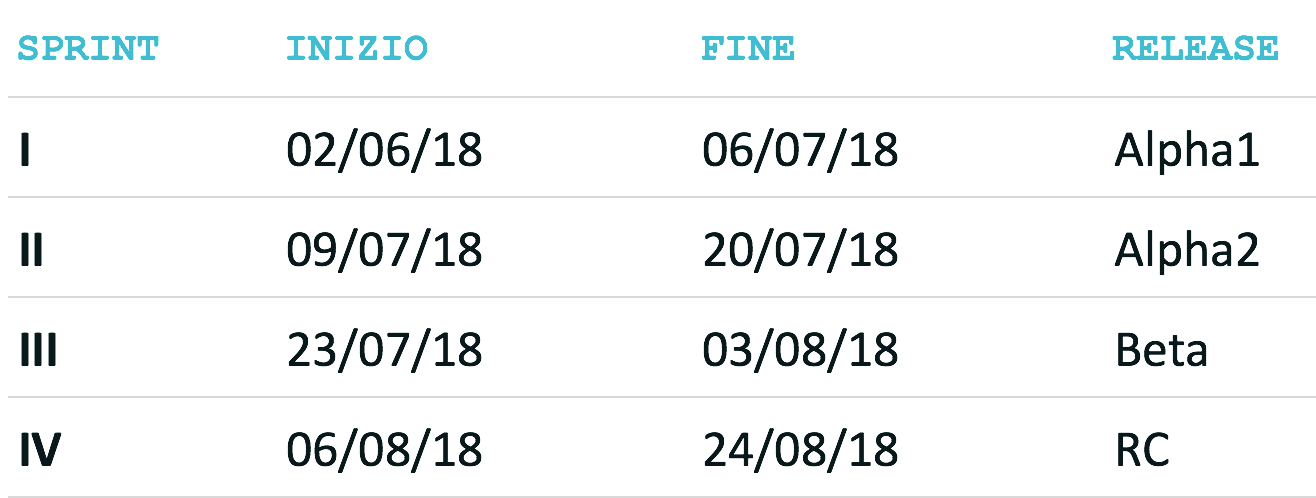
\includegraphics[scale=0.5]{sprint}
	\caption{Definizione sprint}
	\label{fig:sprint}
\end{figure}

\note{mmm fare una tabella decente}

\subsection{I Sprint}
\note{Fare una tabella BELLISSIMA in excel con il riassunto}
Sprint: Alpha 1
\begin{itemize}
	\item Setup progetto (8)
	\begin{itemize}
		\item Expo
		\item TyperScript	
		\item Repo git + submodule OpenChat
		\item Docker + immagine Zimbra\_8.8.8 + ZeXtras
	\end{itemize}
	\item Login
	\item Register session
	\item Strategy
\end{itemize}

\subsection{II Sprint}
\note{Fare una tabella BELLISSIMA in excel con il riassunto}
\subsection{III Sprint}
\note{Fare una tabella BELLISSIMA in excel con il riassunto}
\subsection{IV Sprint}
\note{Fare una tabella BELLISSIMA in excel con il riassunto}
